\documentclass[a4paper]{article}
\usepackage[dutch]{babel}
\usepackage{amsthm,amsmath}
\usepackage{graphicx}
\usepackage{epstopdf}
\usepackage{enumerate}
\usepackage{amssymb}
\usepackage{float}
\usepackage{algpseudocode}
\usepackage{varwidth}
\usepackage{mcode}
\title{Practicum NMB : Eigenwaardenproblemen}
\author{Jona Beysens \& Arnout Devos}
\date{vrijdag 25 apil 2014}

\newcommand{\opgave}[1]{\section*{Opgave #1}}
\newcommand{\dx}{\Delta x}
\newcommand{\dy}{\Delta y}
\newcommand{\dz}{\Delta z}
\newcommand{\dt}{\Delta t}

\begin{document}
\maketitle

\opgave{1}

\begin{algorithmic}
\State Kies $Q^{(0)} \in \mathbb{R}^{m\times d}$ met orthonormale kolommen.
\For {$k = 1,2,...$}
    \State $AZ=Q^{(k-1)}$
    \State $Q^{(k)}R^{(k)}=Z$
    \State $A^{(k)}=Q^{(k)^{T}}AQ^{(k)}$
\EndFor
\State $x = diag(A^{(k)})$
\end{algorithmic}

Dit algoritme is de gelijktijdige inverse iteratie voor het berekenen van de d kleinste eigenwaarden en bijhorende eigenvectoren van de matrix $A$. Het is een aangepaste versie van de gelijktijdige iteratie waarbij gebruik gemaakt wordt van de inverse van $A$. De inverse wordt echter nooit expliciet berekend maar er wordt telkens een stelsel opgelost naar $Z$. De eigenwaarden van $A^{-1}$ zijn de inversen van de eigenwaarden van $A$ en de eigenvector horende bij $\lambda_i$ is dezelfde als die horende bij $\frac{1}{\lambda_i}$:
\begin{proof}
\begin{align}
	Ax &= \lambda x \label{eq1}\\ 
    A^{-1}Ax &= \lambda A^{-1}x \label{eq2}\\
    \frac{1}{\lambda} &= A^{-1}x \label{eq:const1}
\end{align}
\end{proof}
De eigenvectoren horende bij de kleinste eigenwaarden van $A$ komen nu in de eerste kolommen van $Q$ te staan. Daardoor zal $A^{(k)}$ convergeren naar een diagonaalmatrix waarvan de eerste diagonaalelementen de kleinste eigenwaarden van $A$ zijn.

\opgave{2}
\begin{enumerate}[a)] % a), b), c), ...
\item Als $\mu$ een eigenwaarde van $A$ goed benadert, worden de grootste eigenwaarde van $(A-\mu I)^{-1}$ en het conditiegetal van $(A-\mu I)$ zeer groot. Daardoor zal bij het aanleggen van een perturbatie op de matrix $(A-\mu I)$ de oplossing $\hat{y}$ van het stelsel sterk afwijken van het originele probleem. Maar omdat de grootste eigenwaarde zo dominant is, ligt de oplossing van het geperturbeerd probleem $\hat{y}$ bijna in dezelfde richting als $y$. De grootte van $\hat{y}$ verschilt echter sterk van deze van $y$. Door te normaliseren verschillen $\hat{y}$ en $y$ enkel nog in richting. Dit verschil is miniem.
\item Om het residu van $Ax-\rho x$ te minimaliseren lossen we het kleinste kwadratenprobleem op:
\begin{proof}
\begin{align}
\displaystyle\min_{\rho\in\mathbb{R}}\Arrowvert Ax-\rho x \Arrowvert _2 \Leftrightarrow x^{T}(Ax-x\rho) &= 0\label{eq1}\\
 x^TAx &= x^T\rho x \label{eq2}\\
 \rho&=\frac{x^TAx}{x^Tx} \label{eq:const1}
\end{align}
\end{proof}
Deze oplossing voor $\rho$ komt overeen met het Ragleigh quoti\"{e}nt $r(x)$.
\end{enumerate}



\opgave{3}
\begin{enumerate}[a)] % a), b), c), ...
\item 
Aangezien er een schatting voor de eigenvector gegeven is, is de Rayleigh inverse iteratie een geschikte methode om de bijhorende eigenwaarde te vinden. Er dient maar 1 eigenwaarde berekend te worden. Deze methode zal bovendien zorgen snelle convergentie. De verwachte convergentiesnelheid is immers maximaal cubisch. Dit wordt aangetoond in Theorema 27.3 //VERWIJZING//. Om de rekenkost van de iteratie te beperken wordt de symmetrische matrix $A \in \mathbb{R}^{m\times m}$ getransformeerd tot een tridiagonale matrix. Hiervoor wordt Householder triangularisatie gebruikt. In het algemeen bedraagt totale hoeveelheid rekenwerk hiervoor  $10/3*m^3$ flops. Aangezien gebruikt gemaakt kan worden van symmetrie en spaarsheid kan dit werk gereduceerd worden tot $4/3*m^3$ flops. In elke stap van de Rayleigh inverse iteratie moet er een stelsel worden opgelost. Dit bepaalt het meeste werk in elke stap. Dit vraagt in het algemeen $\mathcal{O} (m^3)$ flops. Door gebruik te maken van een vereenvoudigde vorm van Gaussiaanse eliminatie (Thomas Algoritme)kan het rekenwerk gereduceerd worden tot $\mathcal{O} (m)$ flops. Ook wordt de oplossing van het stelsel genormaliseerd. Dit vraagt $n$ flops. Als laatste wordt het Rayleigh quoti\"ent berekend. $A*v$ zorgt voor $5*n$ flops(3 vermenigvuldigingen en 2 optellingen per element). $v^{T}*A*v$ kost dan uiteindelijk nog $2*n-1$ flops($n$ vermenigvuldigingen en $n-1$ optellingen). Het Rayleigh quoti\"ent vraagt dus $7*n-1$ flops. Als convergentie bereikt wordt in $\mathcal{O} (m)$ stappen bedraagt het totale rekenwerk na de tridiagonalisatie dus globaal $\mathcal{O} (m^2)$.

\item
Om de eigenwaarde te bepalen die zich het dichtst bij een getal $alpha$ bevindt, is het QR algoritme met shifts een geschikte methode. het QR algoritme berekent alle eigenwaarden. Hierdoor kunnen we makkelijk zien hoe ver de minder dichte eigenwaarden van $alhpa$ liggen. We kunnen $alpha$ als initi\"ele benadering voor de te zoeken eigenwaarde gebruiken. In elke iteratie kunnen we de benadering verbeteren door het Rayleigh quoti\"ent te nemen. Het QR algortime convergeert maximaal cubisch naar de gezochte eigenwaarde. Het convergeert lineair naar de andere eigenwaarden. Om het rekenwerk te verminderen (zie opgave 4), is ook hier tridiagonalisatie van $A$ vereist. Dit vergt $4/3*m^3$ flops(zie boven). In elke stap van het algoritme moet een QR factorisatie berekend worden. De vector $v$ die nodig is voor het berekenen van de Householder reflector heeft slechts 2 elementen verschillend van 0. Het opstellen van van de reflector vraagt ongeveer $20*n$ flops (2 normen en een deling). Bij het toepassen van de reflectoren op de matrix A worden er door elke reflector ongeveer 5 elementen aangepast. Hiervoor zijn 3 flops per element nodig (2 vermenigvuldigingen en 1 optelling) dus 15 flops in totaal per reflector. Na $n-1$ reflectoren wordt de bovendriehoeksmatrix bekomen dus in totaal zijn er ongeveer $15*(n-1)$ flops vereist. Ook moet er in elke stap van het algoritme $R*Q$ berekend worden. Ook deze bewerking vraagt $\mathcal{O} (m)$ rekenwerk omdat hier de householder reflectoren kunnen gebruikt worden om het product uit te rekenen. Indien convergentie in $\mathcal{O} (m)$ stappen bereikt wordt, zal ook deze methode buiten de tridiagonalisatie in totaal $\mathcal{O} (m^2)$ rekenwerk vragen. 

\item \textbf{JONA} Arnout oplossing: Om, gegeven een symmetrische matrix $A \in \mathbb{R}^{m\times m}$, de eigenwaarde te berekenen die het dichtst bij een getal $\alpha$ gelegen is, kunnen we gebruik maken van \textit{inverse iteratie}. De convergentie is lineair en zal veel sneller gebeuren naarmate $\alpha$ dichter bij de gewilde eigenwaarde gelegen is. De rekenkost is $\mathcal{O} (m^3)$ doordat er een stelsel moet worden opgelost bij het inverteren van de matrix $A-\alpha I$.
\end{enumerate}
De oplossing van opgave 2. Zie figuur~\ref{fig:figure1}.
\opgave{4}
In figuur ~\ref{fig:figure1} zien we de structuur van de matrix \textit{mat1.txt} na reductie naar de Hessenberg vorm. Doordat de matrix niet perfect symmetrisch is, staan er nog waarden in de bovendriehoek die verschillend zijn van 0. Als we kijken naar de grootte van de waarden in die bovendriehoek dan zijn deze allemaal klein. Als we alle waarden die in absolute waarde kleiner dan $10^{-14}$ zijn gelijk aan 0 stellen dan verkrijgen we de vorm in figuur ~\ref{fig:figure2}. Deze tridiagonale vorm is typisch voor reductie van een symmetrische matrix naar een Hessenberg vorm.

\textbf{/////oplossing2/////}\\
Indien de matrix niet gereduceerd zou worden naar Hessenberg vorm, moet in elke iteratie van het QR algoritme de factorisatie berekend worden van een volle matrix. Dit vergt $\mathcal{O}(m^{3})$ flops. De convergentie naar machinenauwkeurigheid $\epsilon _{mach}$ gebeurt meestal in $\mathcal{O}(m)$ stappen wat het totale vereiste werk op $\mathcal{O}(m^{4})$ flops brengt. Het rekenwerk van de QR factorisatie van een matrix in Hessenbergvorm bedraagt $\mathcal{O}(m^{2})$ flops. Hierdoor komt het totale werk op $\mathcal{O}(m^{3})$ flops. Aangezien de Hessenbergvorm van de matrix $mat1.txt$ een tridiagonale vorm heeft zal er zelfs nog minder werk nodig zijn. Het rekenwerk voor een QR factorisatie van een tridiagonale matrix is immers $\mathcal{O}(m)$ flops waarmee het totale rekenwerk op $\mathcal{O}(m^{2})$ flops komt.
\begin{figure}[H]
\begin{minipage}[t]{0.45\linewidth}
\centering
\centerline{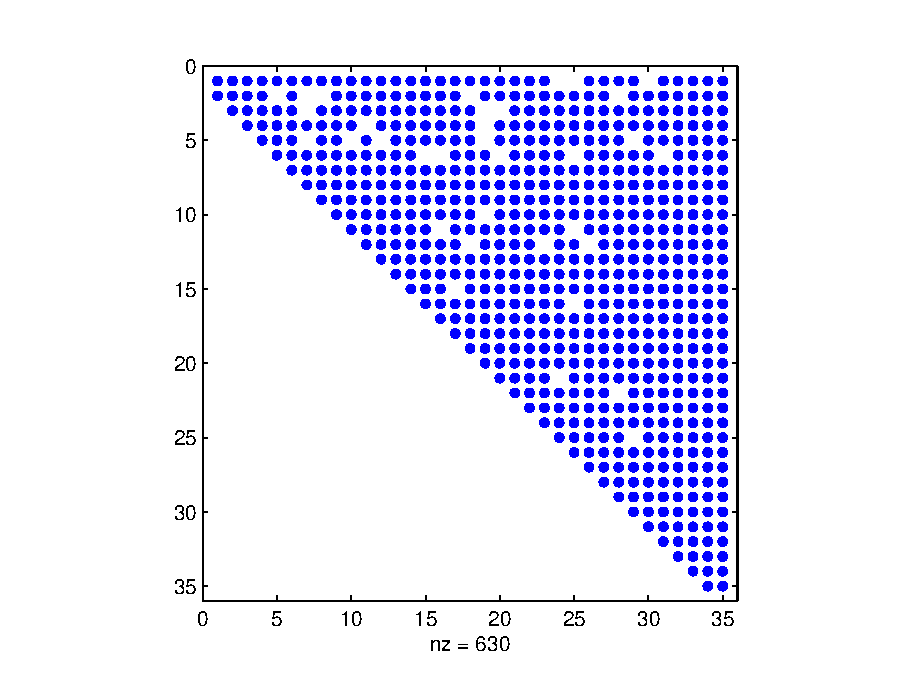
\includegraphics[scale=0.45]{pictures/opgave4Hessenberg1.eps}}
\caption{Vorm van de matrix \textit{mat1.txt} door reductie naar Hessenberg vorm}
\label{fig:figure1}
\end{minipage}
\hfill
\begin{minipage}[t]{0.45\linewidth}
\centering
\centerline{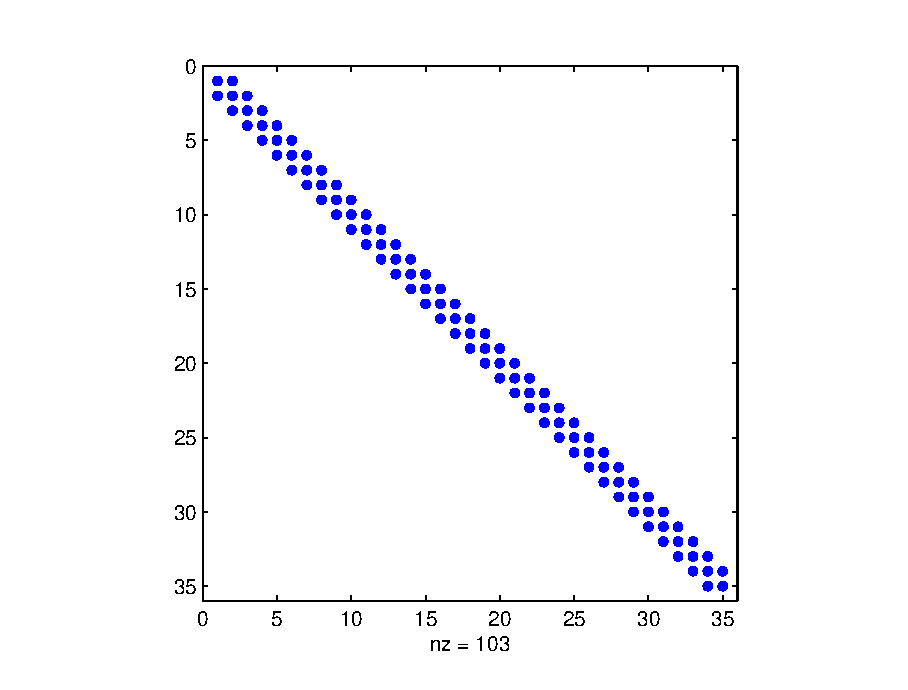
\includegraphics[scale=0.45]{pictures/opgave4Hessenberg2.eps}}
\caption{Tridiagonale vorm van de matrix \textit{mat1.txt} na reductie naar Hessenberg vorm en verwaarlozing van elementen $<10^{-13}$}
\label{fig:figure2}
\end{minipage}
\end{figure}
Indien de matrix niet gereduceerd zou worden naar Hessenberg vorm, moet in elke iteratie van het QR algoritme de factorisatie berekend worden van een volle matrix. Dit vergt $\mathcal{O}(m^{3})$ flops. De convergentie naar machinenauwkeurigheid $\epsilon _{mach}$ gebeurt meestal in $\mathcal{O}(m)$ stappen wat het totale vereiste werk op $\mathcal{O}(m^{4})$ flops brengt. Het rekenwerk van de QR factorisatie van een matrix in Hessenbergvorm bedraagt $\mathcal{O}(m^{2})$ flops. Hierdoor komt het totale werk op $\mathcal{O}(m^{3})$ flops. Aangezien de Hessenbergvorm van de matrix $mat1.txt$ een tridiagonale vorm heeft zal er zelfs nog minder werk nodig zijn. Het rekenwerk voor een QR factorisatie van een tridiagonale matrix is immers $\mathcal{O}(m)$ flops waarmee het totale rekenwerk op $\mathcal{O}(m^{2})$ flops komt.
\opgave{5}
Op figuur ~\ref{fig:opgave5} kunnen we duidelijk zien dat de \textit{QR-methode zonder shift} lineair convergeert wat overeenkomt met de theorie.
\begin{figure}[H]
\centerline{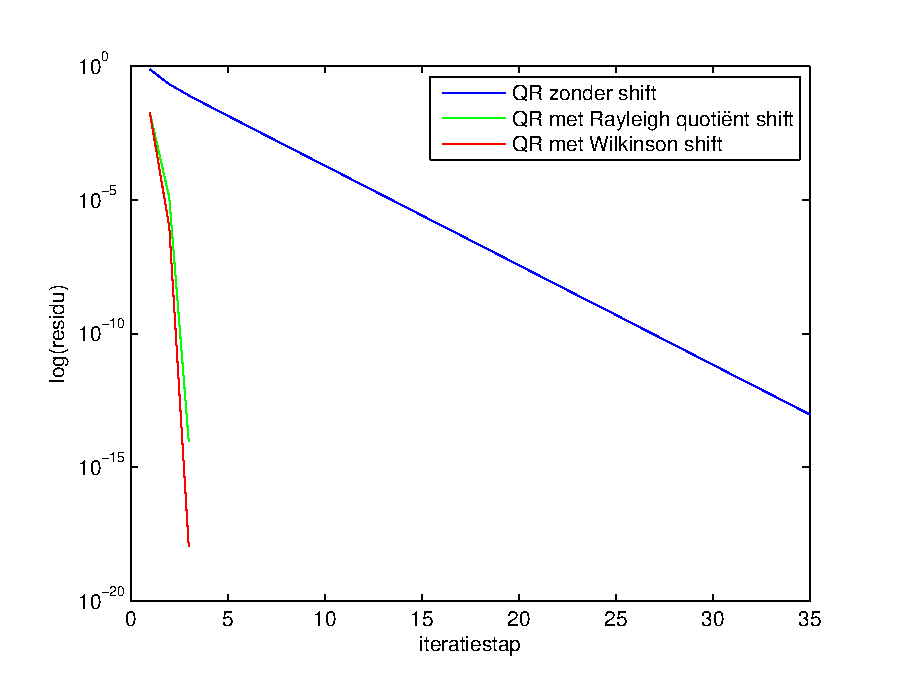
\includegraphics{pictures/opgave5grafiek.eps}}
\caption{Convergentie van de verschillende QR methodes: zonder shift, Rayleigh quoti\"{e}nt shift en Wilkinson shift op logaritmische schaal.}
\label{fig:opgave5}
\end{figure}
In tabel \ref{table:tab2} zien we dat voor de matrix mat1 er voor de \textit{QR iteratie met Rayleigh quoti\"{e}nt shift} en de \textit{QR iteratie met Wilkinson shift} er eerst lineaire convergentie optreedt. Wanneer bij deze algoritmes het residu voldoende klein is geworden, verloopt de convergentie meer en meer kubisch. Dit komt overeen met de theorie die zegt dat $q_m^{(k)}$ kubisch convergeert tot een eigenvector. Daardoo convergeert ook het bijbehorende Rayleigh quoti\"{e}nt $r(q_m^{(k)})=A_{mm}^{(k)}$ kubisch. Naarmate het aantal iteraties toeneemt wordt de invloed van de kubische convergentie steeds groter omdat het aantal elementen dat nog moet convergeren naar een eigenwaarde in elke iteratiestap kleiner wordt.
\begin{table}[h]
\begin{tabular}{|l|l|l|l|}
\hline
stap & zonder shift & Rayleigh quoti\"{e}nt shift & Wilkinson shift \\
\hline
1 & 0.763590501238868 & 0.0183598152348892 & 0.0183598152348892 \\
2 & 0.210113423731095 & 1.23415266649239e-05 & 9.83319921427331e-07 \\
3 & 0.0808375414586785 & 9.55801949807706e-15 & 1.13833614396543e-18 \\
\vdots & \vdots &  &  \\
10 & 0.000192468492953297 &  &  \\
11 & 8.16489243297394e-05 &  &  \\
12 & 3.46381851762602e-05 &  &  \\
13 & 1.46948586913677e-05 &  &  \\
14 & 6.23416040757481e-06 &  &  \\
15 & 2.64479155115201e-06 &  &  \\
16 & 1.12203213434041e-06 &  &  \\
\vdots & \vdots &  &  \\
32 & 1.23546560557316e-12 &  &  \\
33 & 5.24136923576435e-13 &  &  \\
34 & 2.22361119093024e-13 &  &  \\
35 & 9.43350202212816e-14 &  &  \\
\hline
\end{tabular}
\caption{Convergentie van het residu bij de berekening van eigenwaarden volgen verschillende methodes.}
\label{table:tab2}
\end{table}
\opgave{6}
Het verband tussen het \textit{QR-algoritme met Rayleigh quoti\"{e}nt shift} en de \textit{Rayleigh quoti\"{e}nt iteratie}, is dat de veronderstelde waarden voor de eigenvector
en eigenwaarde bij het QR-algoritme, $\mu$ en $q_m^{(k)}$, dezelfde zijn als de waarden
die berekend worden bij de Rayleigh quoti\"{e}nt iteratie met startvector $e_m$. Er wordt dus een Rayleigh quoti\"{e}nt iteratie toegepast op de laatste eigenwaarde van
A. De Rayleigh quoti\"{e}nt iteratie convergeert kubisch, dus de convergentie van het QR algoritme met Rayleigh shift moet ook kubisch zijn. De Rayleigh shift heeft geen invloed op de andere eigenwaarden, dus er wordt verwacht dat deze lineair convergeren net als bij gelijktijdige iteratie het geval is.
//////EXTRA INFO HIER NOG + VB FIGUUR/////
\opgave{7}
Als men de \textit{Arnoldi} methode gebruikt op een ijle matrix $A \in \mathbb{R}^{1000\times1000}$ en de Ritz waarden per iteratiestap uitzet dan verkrijgt men Figuur ~\ref{fig:opgave7}.
Wat opvalt aan het convergentiegedrag is dat wanneer een Ritz waarde in de buurt komt van een eigenwaarde, ze alleen nog dichter bij de eigenwaarde zal gaan liggen in de volgende iteratiestappen. Vroege convergentie is te zien aan de lange rode lijnen die dus niet meer afwijken van een bepaalde waarde. Het convergentiegedrag is lineair en versnelt wanneer er meer eigenwaarden gevonden zijn.
\begin{figure}
\centerline{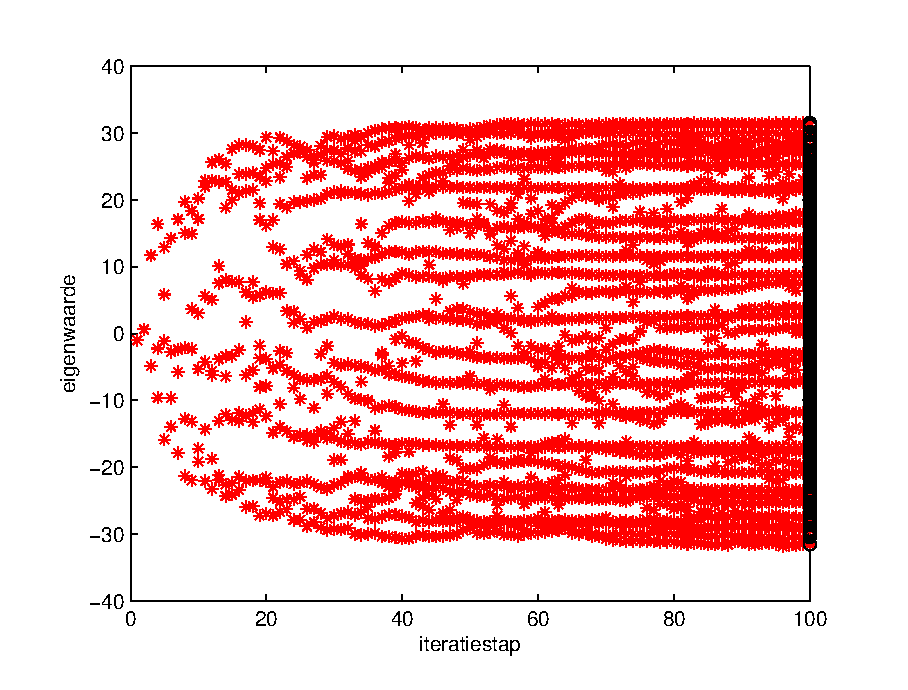
\includegraphics{pictures/opgave7.eps}}
\caption{Convergentie van de Ritz waarden (rode kruisjes) naar de echte eigenwaarden van A (zwarte cirkels).}
\label{fig:opgave7}
\end{figure}
\opgave{9}
Dit is de code van matlab:
\lstinputlisting{opgave_9.m}
\end{document}
